\chapter{Modeling the Effects of Feedback}
\label{chapter:modeling}

% \subsection{Model Extension}
% The third and final Aim of the proposal is addressed by developing a model of the human pilot which includes the effects of concurrent bandwidth feedback.
% The proposed Model will extend Professor Hess' structural model of the human pilot to include the effects of concurrent bandwidth feedback.
% The Structural Model has been extremely successful in predicting human performance through a variety of system dynamics and can predict how performance changes during a pilot's adaptation to changing dynamics.
% Hess has developed adaptive logic for the human pilot in a pursuit task which triggers when the pilot notices that vehicle dynamics have changed~\citep{hess_modeling_2009}.
% This logic is based off several criteria, which ``must be predicated upon information available to the human [and] the postadapated pilot models must follow the dictates of the crossover model of the human pilot~\citep{hess_modeling_2009}.''
% The primary result of the adaptive logic is to increase the resulting crossover frequency of the pilot, effectively making them more responsive, which could be interpreted as more focused on the task.
% Our initial approach to adding concurrent bandwidth feedback into the Structural Model will be based off of Hess' approach to modeling human adaptation in pursuit tasks, which is currently ad-hoc in nature, see Figure~\ref{figure:hesspursuit}.

% \begin{figure}[tb]
%     \begin{center}
%         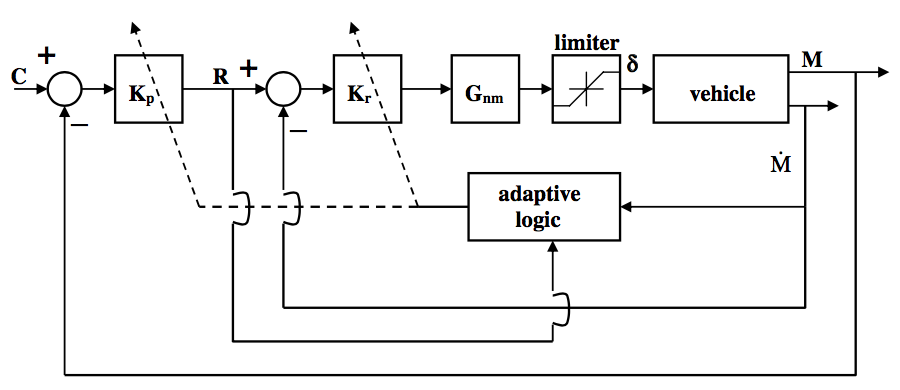
\includegraphics[width=0.8\linewidth]{figures/Screen_Shot_2018-08-09_at_4_15_24_PM.png}
%         \caption[Hess' model of the adaptive human pilot.]{Hess' model of the adaptive human pilot, from~\citep{hess_modeling_2009}.}
%         \label{figure:hesspursuit}
%     \end{center}
% \end{figure}

% While this model of the adaptive pilot has been successful in predicting changes in performance for a well trained subject, it does not consider how a pilot would behave when they are still in the early stages of training.
% Our modified model will include two major changes to Hess' current model:
% \begin{itemize}
%     \item The adaptation logic will be changed to focus on concurrent bandwidth feedback
%     \item The timescale of the adaptation will be significantly longer
% \end{itemize}

% We propose to modify the adaptive logic to trigger when the pilot is receiving concurrent bandwidth feedback, rather than when a change in system dynamics occurs.
% This will require the addition of a feedback loop onto the Structural Model which triggers when the bandwidth feedback is activated.
% This loop will likely be based around the $K_e$ gain, which is currently the primary way of setting the crossover frequency in the Structural Model.
% This implies that the subjects in our experiments do their primary learning when they are receiving qualitative feedback that their current level of aggressiveness is not sufficient to complete the task.
% While there must be a separate loop that adjusts the crossover frequency as learning progresses over the course of several hours, the change in performance we see when subjects use the concurrent bandwidth feedback happens relatively rapidly, within a few minutes.
% This is reflected in the delta of performance between subjects in the different groups of our SAFER experiment, even on the first trial, see Figure~\ref{figure:saferdistance}.
% This relates to the second required change, the amount of required adaptation time.
% Professor Hess' model requires that pilots adapt within a very short time period, on the order of 5 seconds~\citep{weir_model_1966}.
% The results of our experiment with SAFER and the three-axis tracking task also suggest relatively short adaptation times, though they are on the order of a few minutes, again see Figure~\ref{figure:saferdistance}.

% While it should be noted that this work is in preliminary stages and not scheduled to begin until the Fall Quarter, some early work has been started in preparation for the qualifying examination.
% An effort has been made to begin to replicate some of Hess' results.
% Working with Professor Hess, we have been able to replicate some of the existing adaptation logic for a two-axis tracking task, and begun exploratory research into modifying the model.

% \begin{document}
% \title{Pilot Model Approaches for Interpreting the\\Effects of Concurrent Feedback}

% \begin{abstract}
% \chapter{IEEE Paper That Was Not}
We want to use models to identify some aspect(s) which cause the pilot to perform better.

Training operators to perform complex manual control tasks is expensive and time consuming, and poorly trained operators can cause catastrophic failures.
The use of concurrent feedback techniques has been shown to improve performance and reduce training times, but has not been evaluated for complex, real-world tasks such as flying aircraft.
Thirty participants were evenly split into two groups and tasked with flying a simulated Boeing 747 aircraft in three control modes of increasing degrees of freedom and functional complexity.
The control group controlled simulated aircraft motion with visual guidance for pitch, roll, and altitude provided by traditional flight instruments.
The feedback group received additional visual concurrent feedback for each controlled degree of freedom.
For both groups, performance measurements were evaluated to determine the effects of the feedback on subject learning rate and maximum skill level.
To assess short-term retention of learned skill for the feedback group, the concurrent feedback was removed, and performance was again evaluated.

A time-domain autoregressive exogenous (ARX) identification technique was used to estimate pilot transfer functions and the estimated pilot/vehicle open-loop transfer functions were evaluated to determine the evolution of the crossover frequency for each control loop throughout training.
The Hess Structural Model of the pilot is also investigated, which “describe the underlying structure which contributes to human pilot dynamics.'' The Structural Model is of interest for interpreting the effects of concurrent feedback as it incorporates multiple sensory channels and models of visual acuity and the time-varying human pilot.
Results indicate that participants in the feedback group had a significantly lower root-mean-square error and higher crossover frequency than those in the control group, indicating better performance.
The ARX identification technique provided a consistently high variance accounted for (VAF), indicating that it can identify transfer functions representing a variety of operators at various levels of training.
These results are more pronounced for modes with increased functional complexity and persisted in retention testing when the feedback was removed, indicating that participants were not reliant on the feedback.
% \end{abstract}

% \tableofcontents

\section{Introduction}
Extrinsic feedback, which is also known as augmented feedback, has been extensively studied in the field motor learning.
In their 2013 review, Sigrist et al. write ``[i]t is generally accepted that augmented feedback, provided by a human expert or a technical display, effectively enhances motor learning''~\cite{sigrist_augmented_2013}.
There are a variety of different forms of augmented feedback, that can be further classified by how, when, and by what form the feedback is provided.
For this work, however, we sought to evaluate a type of feedback which was both conceptually simple and could be tied to operational requirements.
With these requirements in mind, we investigated the effects of concurrent bandwidth feedback.
Concurrent, or real-time, feedback is displayed to the operator while the task is being executed, in contrast to terminal feedback, which is displayed after the task is complete.
Bandwidth feedback is displayed to the operator when some parameter is inside (on-track feedback) or outside (off-track feedback) of an acceptable, predefined tolerance limit.
In our implementation, concurrent bandwidth feedback describes feedback conveyed to the operator when their real-time performance drifts outside of an acceptable tolerance limit.

Early control theory based models of human operators were summarized in McRuer's 1957 report, ``Dynamic Response of Human Operators''~\cite{mcruer_dynamic_1957}, which evaluated measurements for single-input/single-output manual control systems and developed predictive models consistent with this data.
The report concludes by describing a transfer function of the human operator which includes a time delay, a neuromuscular lag, and a gain.
McRuer revisited these results in 1974, after three decades of supporting engineering and experimental psychology experiments and was able to further generalize these results to a wide variety of system dynamics~\cite{mcruer_mathematical_1974}.
The result of this report was the now famous ``crossover model,'' which relates the operator and controlled element transfer characteristics by the equation
\begin{equation}
    Y_c(jw) Y_p(jw) = \dfrac{w_c e^{-jw \tau_e}}{jw}
\end{equation}
where $Y_c$ is the controlled element transfer function, $Y_p$ is the approximate human operator transfer function, $w_c$ is the crossover frequency, and $\tau_e$ is the effective time delay of the pilot.
The crossover model is so named as it allows for linear behavior at approximately -20 dB/decade slope in the region of the crossover frequency.
Modeling the human pilot with the crossover enables a more complete view of the complete pilot/vehicle system, and allows for human factors recommendations towards the design of new vehicles.
The crossover model is used as the standard for describing pilot/vehicle systems at the crossover frequency~\cite{mcruer_mathematical_1974,mcruer_human_1965,xu_review_2017}.

The continued demand for human pilot models for use in informing vehicle design, as well predicting, preventing, and explaining accidents has led to a variety of more complex pilot models since the creation of the crossover model.
A recent review by Xu et al. in 2017 surveyed the state of the art in human pilot modeling and grouped existing models into three classes of models based on: control theory, human physiology, and intelligence techniques~\cite{xu_review_2017}.
Classical models based on control theory include the McRuer crossover model and optimal control models by Kleinman et al. developed in the early 1970s~\cite{kleinman_optimal_1970,baron_optimal_1970}.
Of these three overarching sets of models, the models based on human physiology are of the greatest interest here.
Models based on human physiology were developed to understand human pilot perception and control behavior, and include the Hess structural model~\cite{hess_structural_1980,hess_model_1990,hess_unified_1997}, Hosman's descriptive model~\cite{hosman_pilots_nodate,hosman_pilots_1999}, and the biodynamic model~\cite{griffin_validation_2001}.
Recent intelligence models take advantage of techniques including fuzzy control and neural networks~\cite{zaychik_conspectus_2006,gestwa_modelling_2003}.

% \begin{figure}[t]
%     \centering
%     \begin{subfigure}[b]{0.49\textwidth}
%         \centering
%         \includegraphics[width=\textwidth]{figures/structural_model/structural_model.pdf}
%         \caption{The complete Structural Model, from~\cite{hess_unified_1997}.}
%         \label{fig:structuralmodel}
%     \end{subfigure}
%     \hfill
%     \begin{subfigure}[b]{0.49\textwidth}
%         \centering
%         \includegraphics[width=\textwidth]{figures/structural_model_reduced/structural_model.pdf}
%         \caption{The reduced structural model used in this analysis.}
%         \label{fig:structuralmodelreduced}
%     \end{subfigure}
%     \caption{The Structural Model of the Human Pilot.}
%     \label{fig:structuralmodels}
% \end{figure}

While the McRuer was very successful in predicting pilot behavior, it it did not attempt ``to describe the underlying structure which contributes to human pilot dynamics~\cite{hess_structural_1980}.''
For this reason, the Structural Model is of particular interest due to the incorporation of multiple sensory channels and models of visual acuity and the time-varying human pilot~\cite{hess_modeling_2009}.
The Structural Model includes the effects of the neuromuscular system, the force-feel characteristics of the input device, and the contributions of proprioceptive, vestibular, and visual feedback, see Figure~\ref{fig:structuralmodels}.
One of the key strengths of the Structural Model is the relatively few number of free parameters that need to be set to predict pilot performance.
The model has been used in predicting and evaluating handling qualities and pilot-induced oscillation rating levels for helicopters, Boeing 747, Lockheed C-5A, and twin ducted-fan aircraft~\cite{hess_analytical_2013,andreea-irina_prediction_2014,grant_handling_2015}.
Hess has also investigated how pilot control characteristics change with time due to flight anomalies, changing flight dynamics, and sudden increases in task demand~\cite{hess_modeling_2009,hess_modeling_2016}.
The results of this model have been compared to the results of a human-in-the-loop simulation for a well trained subject, and showed good comparison~\cite{hess_modeling_2016}.
Recent work from Bachelder et al. has included modifications to the Structural Model to link pilot performance and workload and to enable the modeling of pulsive pilot behavior~\cite{bachelder_modeling_2017,bachelder_linking_2018}.

\section{Pilot Modeling Techniques}
We have a ``black box'' model which can give us a coarse understanding of the pilot.
This is the ARX technique which Professor Hess has used, \textit{gettf1}.
We also have the control theory based model, the Structural Model, which Professor Hess has used for several decades.
This model is more interesting because it has multiple parameters which could be responsible for the observed change in performance.

\subsection{AutoRegressive Models with eXogenous Variables (ARX)}
This is the ARX technique which Professor Hess has used, \textit{gettf1}.

\subsection{The Structural Model}
%

\section{Method}

\subsection{The Task}

\begin{figure}[b]
    \centering
    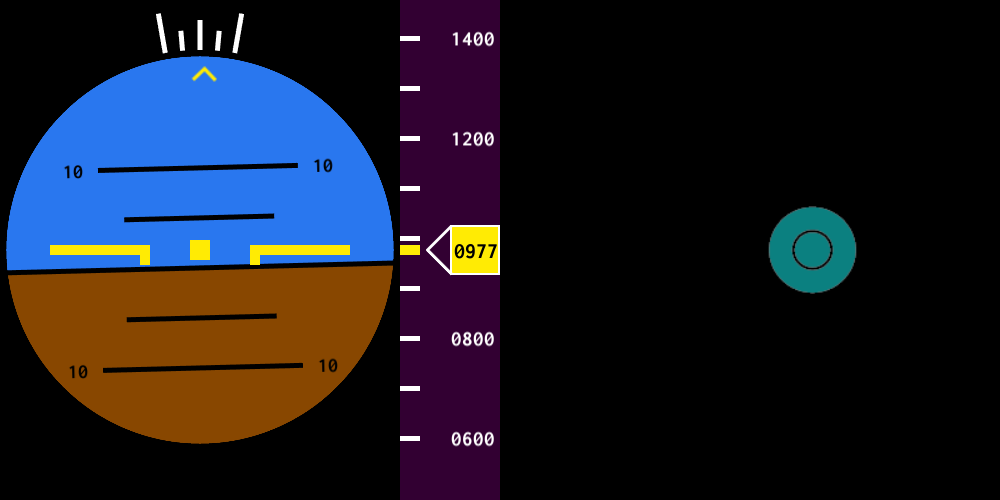
\includegraphics[width=3.25in]{figures/image1.png}
    \caption{The interface that participants were presented with during the experiment, showing the flight task on the right with deviations from nominal in pitch, roll, and altitude, and the secondary, two-choice, task on the right.}
    \label{fig:display}
\end{figure}

Thirty participants were randomly split into two groups and tasked with flying a simulated Boeing 747 aircraft in three control modes. In order of increasing degrees of freedom and functional complexity, these three control modes were:
\begin{itemize}
    \item Pitch only (low complexity)
    \item Pitch and Roll (moderate complexity)
    \item Pitch, Roll and Altitude (significant complexity)
\end{itemize}
Each participant completed a total of 36 trials; 12 in each of the three control modes.
Each trial had a duration of 82 seconds, and participants self-initiated the trial by activating a trigger on the joystick.
The complete results of this experiment can be seen in our HFES paper~\cite{RN42}.

The two groups of participants are: control and feedback, and the interface that participants saw during the experiment is available in Figure~\ref{fig:display}.
When the vehicle was well controlled (small errors in the controlled degrees of freedom), the interface was the same for participants in both groups.
Depending on the control mode the the participant was completing, however, participants in the feedback group experienced concurrent bandwidth feedback on various elements of the attitude indicator and altimeter.
This feedback was indicated by changing the element from the default yellow color to a red color when the error deviated outside of a predetermined bandiwdth.
Pitch feedback was provided on the central pitch indicator when the pitch was three or more degrees from zero, roll feedback was provided on the attitude indicator's ``wings'' when the roll was three or more degrees from zero, and attitude feedback was provided on the altimeter text box when the altitude was 30 feet or more off the nominal altitude of 1000 feet.
After the 9th trial, subjects in the feedback group no longer experienced feedback, and the interfaces for the control and feedback groups were the same.
This was done in order to investigate how well the subjects could retain their performance benefit.

The resulting root-mean-square error for each group of participants by trial is presented in Figure~\ref{fig:prmse}.
Both groups of participants had a relatively high initial RMSE which was reduced through repeated training on the task.
Participants in the feedback group, however, performed significantly better than those in the control group and learned the task much faster.
Additionally, subjects in the feedback group were able to maintain their improved performance when the feedback was removed, and actually show a slight increase in performance when this occurs.

\begin{figure}[t]
    \centering
    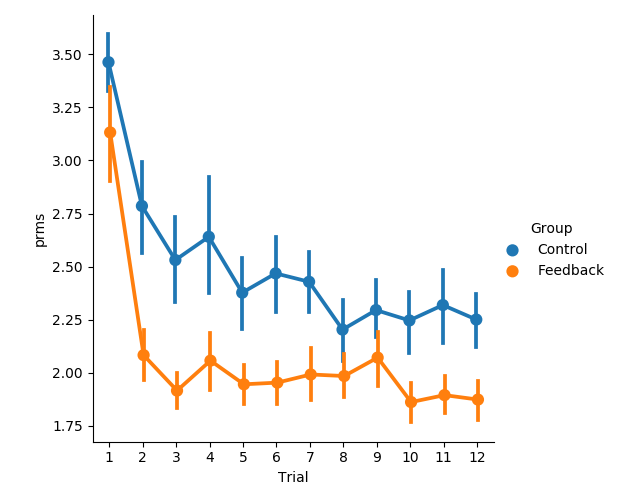
\includegraphics[width=3.25in]{figures/model_prms.png}
    \caption{Pitch root-mean-square error. Feedback was removed from subjects in the feedback group after the 9th trial in order to investigate retention.}
    \label{fig:prmse}
\end{figure}

\subsection{ARX Model Identification}
This is pretty simple, we simply pass the input/output data into gettf1 and observe the characteristics of the resulting transfer function.
We can also combine the estimated operator transfer function with the vehicle dynamics to observe the overall system characteristics, such as the crossover frequency.

An autoregressive technique to identify a transfer function from an input/output time sequence pair was previously developed by Hess et al.~\cite{hess_modeling_2002}.
Using this technique, called \textit{gettf1}, we identified transfer functions representing pilot models for the data trials from our experiment.
The resulting pilot models can be compared with the experimental data from which they are generated in order to determine the goodness of fit.
Two goodness of fit metrics are available: the variance accounted for (VAF) and the root-mean-square error between the model output and participant data.
The VAF is calculated by
\begin{equation}
    \mbox{VAF} = \left( 1 - \dfrac{\sum{|u - u_{sim}|^2}} {\sum{u^2}} \right) \times \mbox{100\%}
\end{equation}
where $u$ is the participant's command input to the vehicle's elevators, and $u_{sim}$ is the model's simulated input.

% \begin{figure}
%     \centering
%     \begin{subfigure}[b]{0.49\textwidth}
%         \centering
%         \includegraphics[width=\textwidth]{../../Analysis/figures/model_vaf.png}
%         \caption{Variance accounted for (VAF).}
%         % \label{fig:y equals x}
%     \end{subfigure}
%     \hfill
%     \begin{subfigure}[b]{0.49\textwidth}
%         \centering
%         \includegraphics[width=\textwidth]{../../Analysis/figures/model_rmserr.png}
%         \caption{Root-mean-square error.}
%         % \label{fig:three sin x}
%     \end{subfigure}
%        \caption{Goodness of fit metrics. Error bars are standard error of the mean.}
%        \label{fig:goodnessoffit}
% \end{figure}

\begin{figure}[h]
    \centering
    \begin{subfigure}[b]{0.49\textwidth}
        \centering
        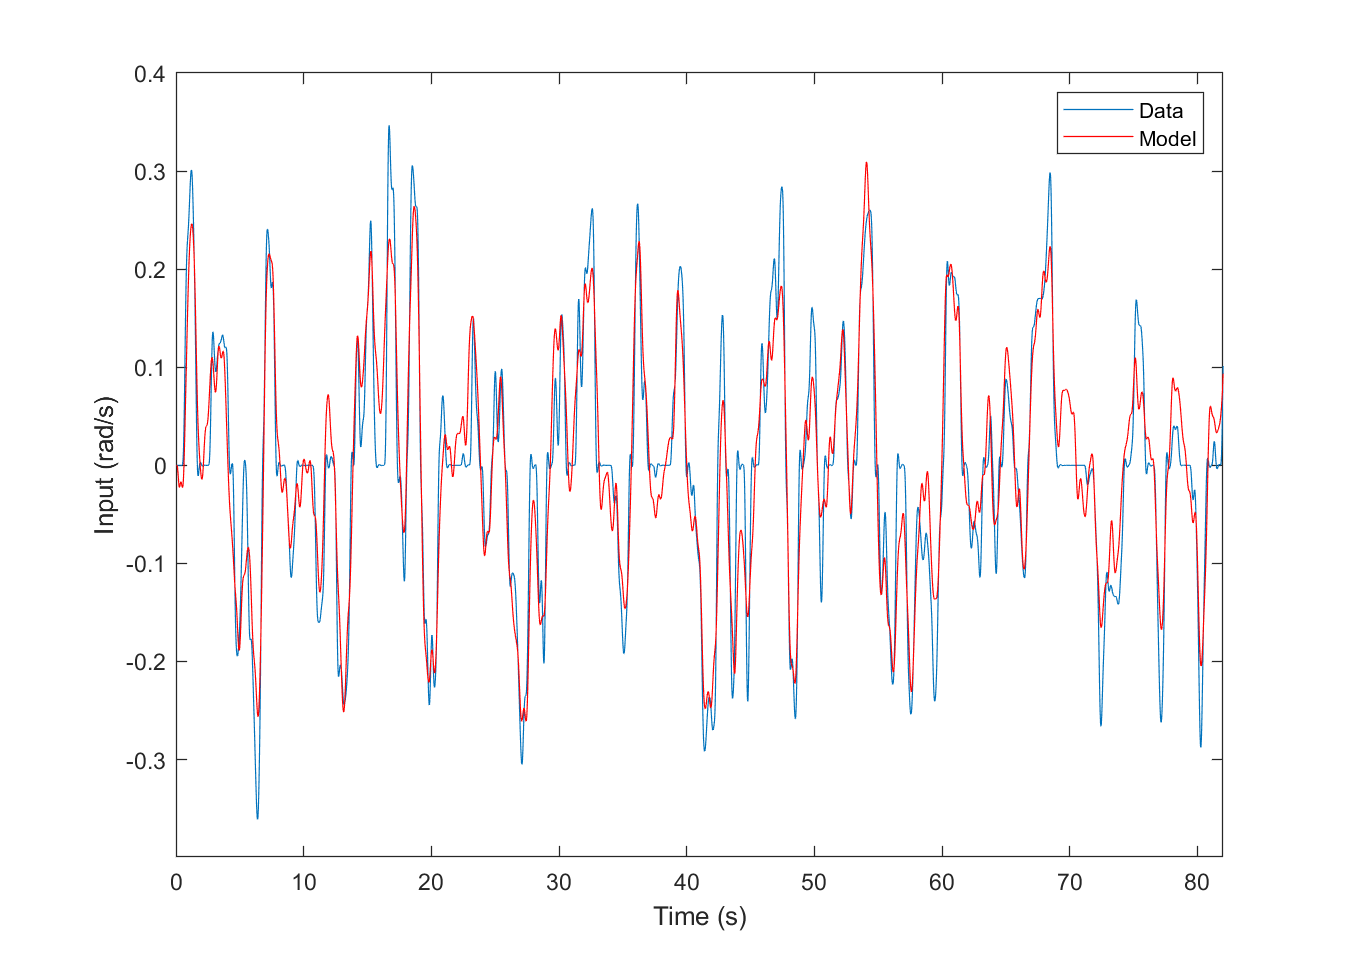
\includegraphics[width=\textwidth]{figures/model_output.png}
        \caption{Comparison between estimated transfer function model and experimental data.}
        \label{fig:comparison}
    \end{subfigure}
    \hfill
    \begin{subfigure}[b]{0.49\textwidth}
        \centering
        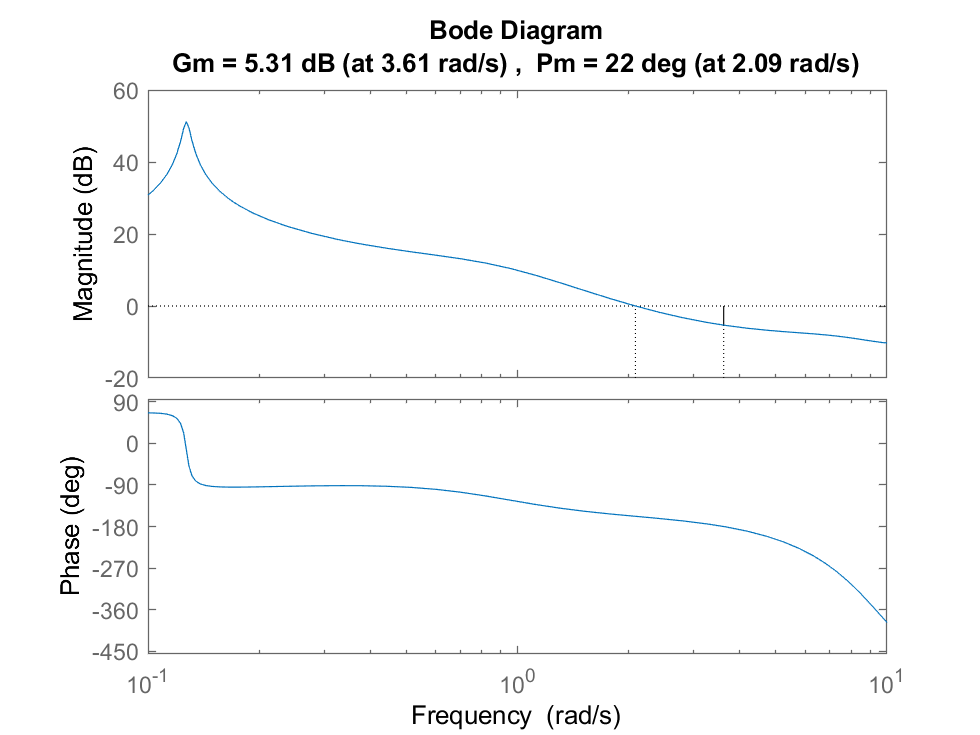
\includegraphics[width=\textwidth]{figures/YpYc_204.png}
        \caption{Combined pilot/vehicle open-loop bode diagram showing the standard crossover model characteristics.}
        \label{fig:bode}
    \end{subfigure}
    \caption{Example results from using the estimated pilot models from \textit{gettf1}.}
    %    \label{fig:goodnessoffit}
\end{figure}

% Both metrics are available in Figure~\ref{fig:goodnessoffit}.
The VAF of the feedback group's models immediately jumps up after the first trial to an average of $\approx.75$, indicating a good fit.
The control groups VAF increases more slowly, to a value of approximately $\approx.68$.
An increased VAF indicates that the pilot is behaving in a more linear fashion, and these results suggest that the concurrent feedback is able to immediately assist participants to this end.
The RMSE between the simulated and actual data is similar between groups and trends slightly up during training.
Visual inspection of the experimental and simulated data also shows very good agreement, see Figure~\ref{fig:comparison}.

By combining these pilot models with the system dynamics the crossover frequency (Figure~\ref{fig:bode}) and gain and phase margins can be found.
The crossover model has long been used as the standard model for human control tasks, where the crossover frequency represents ``how hard'' the pilot is working~\cite{mcruer_dynamic_1957}.
The results of these parameters reflect what was found in the pitch RMSE performance analysis.
Subjects in the feedback group immediately show increased crossover frequency and decreased phase and gain margins.
These results are sustained during retention, and again show an immediate increase/decrease when the feedback is removed.

\begin{figure}
    \centering
    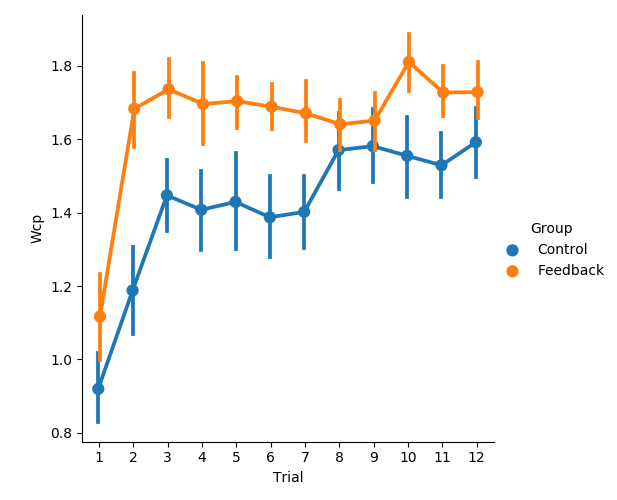
\includegraphics[width=3.25in]{figures/model_Wcp.png}
    \caption{Crossover frequency.}
    \label{fig:crossover}
\end{figure}

Mixed models were used to calculate the significance of factors in our analysis due to the presence of performance outliers which were removed from the analysis.
The Satterthwaite method was used to calculate the adjusted degrees of freedom using the lmerTest package in R~\cite{RN53}.
When significant effects were observed, post hoc comparisons using the Tukey Honest Significance Difference (HSD) test were performed and considered significant at the $p < .05$ level, and the Satterthwaite method was again used to calculate the degrees of freedom.
Only 7 of the 1080 total trials (30 subjects with 36 trials per subject) were removed.
These trials were extreme performance outliers, and including these trials does not change the primary results of the study.

A three-factor (Group, Mode, and Trial) mixed model with two repeated measures (Mode and Trial) was run on the pitch crossover frequency.
There were significant main factors of group $(F(1, 28.00) = 4.9, p = 0.036)$, mode $(F(2, 55.62) = 17.1, p < .001)$, and trial $(F(11, 306.23) = 39.4, p < .001)$.
There were also significant interaction effects between group and trial $(F(11, 306.23) = 2.0, p = 0.025)$ and between mode and trial $(F(22, 610.08) = 2.8, p < .001)$.
Despite the presence of interaction effects that result from participants learning the task (as indicated by the trial factor), the main effects can still be interpreted.
A Tukey test showed that the participants in the groups differed significantly, with the participants in the feedback group outperforming those in the control group $(M = 1.25, 1.56,$ respectively, $SE = 0.10)$.
An additional Tukey test showed that the participants' crossover frequency between the modes differed significantly, with the largest crossover frequency in the P mode, followed by the PR mode, and finally the lowest in the PRA mode $(M = 1.53, 1.38, 1.31$ respectively, $SE = 0.07)$.
This same analysis was completed on the roll crossover frequency, with similar results.
There were significant main factors of group $(F(1, 27.82) = 8.2, p < 0.01)$, mode $(F(1, 25.49) = 23.2, p < 0.001)$, and trial $(F(11, 292.40) = 16.3, p < .001)$.
Tukey tests showed that the participants' crossover frequency between the groups and the modes each differed significantly, with the participants in the feedback group again outperforming those in the control group $(M = 0.55, 0.89,$ respectively, $SE = 0.08)$, and crossover frequency was best in the PR mode followed by the PRA mode $(M = 0.77, 0.67,$ respectively, $SE = 0.06)$.
A two-factor (Group and Trial) mixed model with one repeated measure (Trial) was run on the altitude crossover frequency.
There were significant main factors of group $(F(1, 27.92) = 4.4, p = 0.046)$ and trial $(F(11, 301.95) = 18.3, p < .001)$.
Tukey tests showed that the participants' crossover frequency between the groups differed significantly, with the participants in the feedback group again outperforming those in the control group $(M = 0.98, 1.29,$ respectively, $SE = 0.11)$, and the trial effect showing learning throughout the experiment for both groups.

% \begin{figure}
%     \centering
%     \begin{subfigure}{3.25in}
%         \centering
%         \includegraphics[width=\textwidth]{../../Analysis/figures/model_Gm.png}
%         \caption{The gain margin.}
%         % \label{fig:y equals x}
%     \end{subfigure}
%     \\
%     \begin{subfigure}{3.25in}
%         \centering
%         \includegraphics[width=\textwidth]{../../Analysis/figures/model_Pm.png}
%         \caption{The phase margin.}
%         % \label{fig:three sin x}
%     \end{subfigure}
%        \caption{Characteristics of the open-loop pilot/aircraft transfer function.}
%        \label{fig:gainphase}
% \end{figure}

\subsection{Structural Model Parameter Identification}
This is more complicated, as there are many parameters to identify which interact nonlinearly, and the fit function has many local maximums.

\section{Results}

\begin{figure}[h]
    \centering
    \begin{subfigure}[b]{0.49\textwidth}
        \centering
        \includegraphics[width=\textwidth]{figures/structural_model/structural_model.pdf}
        \caption{The complete Structural Model, from~\cite{hess_unified_1997}.}
        \label{fig:structuralmodel}
    \end{subfigure}
    \hfill
    \begin{subfigure}[b]{0.49\textwidth}
        \centering
        \includegraphics[width=\textwidth]{figures/structural_model_reduced/structural_model.pdf}
        \caption{The reduced structural model used in this analysis.}
        \label{fig:structuralmodelreduced}
    \end{subfigure}
    \caption{The Structural Model of the Human Pilot.}
    \label{fig:structuralmodels}
\end{figure}

\subsection{Model Parameterization}
\begin{equation}
    Y_{NM} = \frac{\omega^2_{NM}}{s^2 + 2 \zeta_{NM} \omega_{NM} s + \omega^2_{NM}}
\end{equation}

\begin{equation}
    Y_{FS} = \frac{\omega^2_{FS}}{s^2 + 2 \zeta_{FS} \omega_{FS} s + \omega^2_{FS}}
\end{equation}

\begin{equation} \label{eq:ypf}
    Y_{PF} = \frac{K}{s+a}
\end{equation}
Equation~\ref{eq:ypf} is chosen to satisfy $Y_{PF} \propto s Y_c (s)$.

\begin{equation}
    Y_{FS} = \frac{\omega^2_{FS}}{s^2 + 2 \zeta_{FS} \omega_{FS} s + \omega^2_{FS}}
\end{equation}

\subsection{Parameter Value Selection}

\begin{equation}
    K_{\dot{e}} = \epsilon = K_{\dot{m}} = K_{\ddot{m}} = 0
\end{equation}

\begin{equation}
    S_1 = S_2 = S_3 = \enspace \downarrow
\end{equation}

\begin{equation}
    \omega_{NM} = 10 \mbox{ rad/s}, \quad \zeta_{NM} = 0.707
\end{equation}

\begin{equation}
    \omega_{FS} = 25 \mbox{ rad/s}, \quad \zeta_{FS} = 0.707
\end{equation}

% \begin{equation}
% Y_c = \frac{0.5716 (s+0.5535) (s+0.03952)}{(s^2 + 0.006158s + 0.01512) (s^2 + 1.12s + 0.8006)}
% \end{equation}

\subsubsection{Value Identification Technique}
A brute force parameter search was used to identify the value of the remaining parameters.
Each combination of the parameters $K_e, \tau_0, K,$ and $a$ were enumerated over and simulated in Simulink using the same flight model and disturbance profiles as the participants experienced in the experiment.
The resulting 55,575 simulations were compared to each trial to identify the set of parameter values resulting in the smallest VAF.

\begin{align}
    K_e    & = [1, 2, 3, \ldots, 25]             \\
    \tau_0 & = [.100, .125, .150, \ldots, 3.0] s \\
    K      & = [1.0, 1.5, 2.0, \ldots, 10.0]     \\
    a      & = [.0, .25, .50, \ldots, 3.0]
\end{align}

\begin{figure}[h]
    \centering
    \begin{subfigure}[h]{0.49\textwidth}
        \centering
        \includegraphics[width=3.25in]{figures/wcp.png}
        \caption{Crossover frequency.}
        \label{fig:sm_crossover}
    \end{subfigure}
    \hfill
    % \begin{subfigure}[h]{0.49\textwidth}
    %     \centering
    %     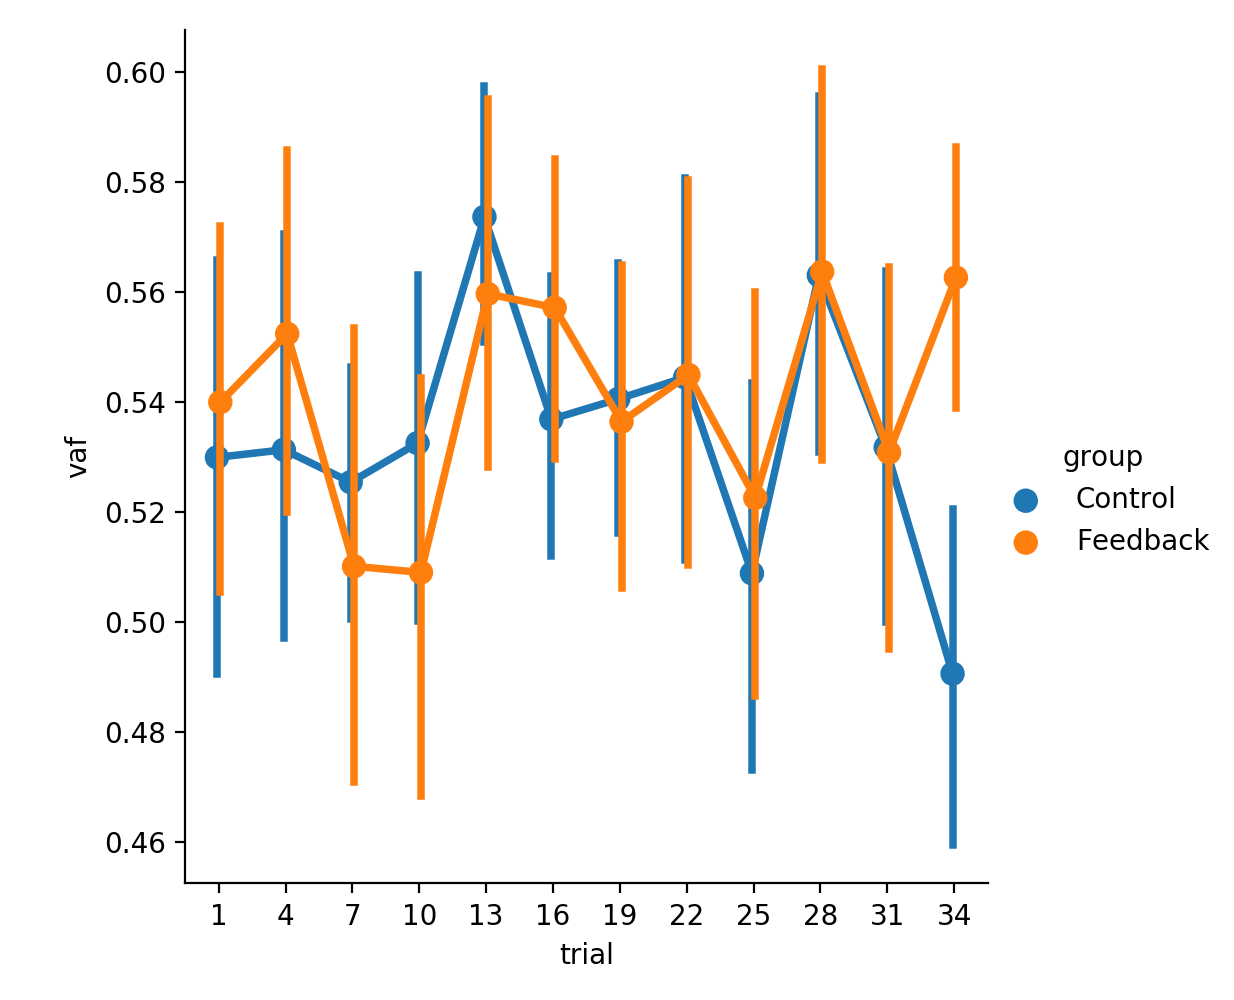
\includegraphics[width=3.25in]{figures/vaf.png}
    %     \caption{Variation-accounted-for.}
    %     \label{fig:sm_vaf}
    % \end{subfigure}
    % \hfill
    \begin{subfigure}[h]{0.49\textwidth}
        \centering
        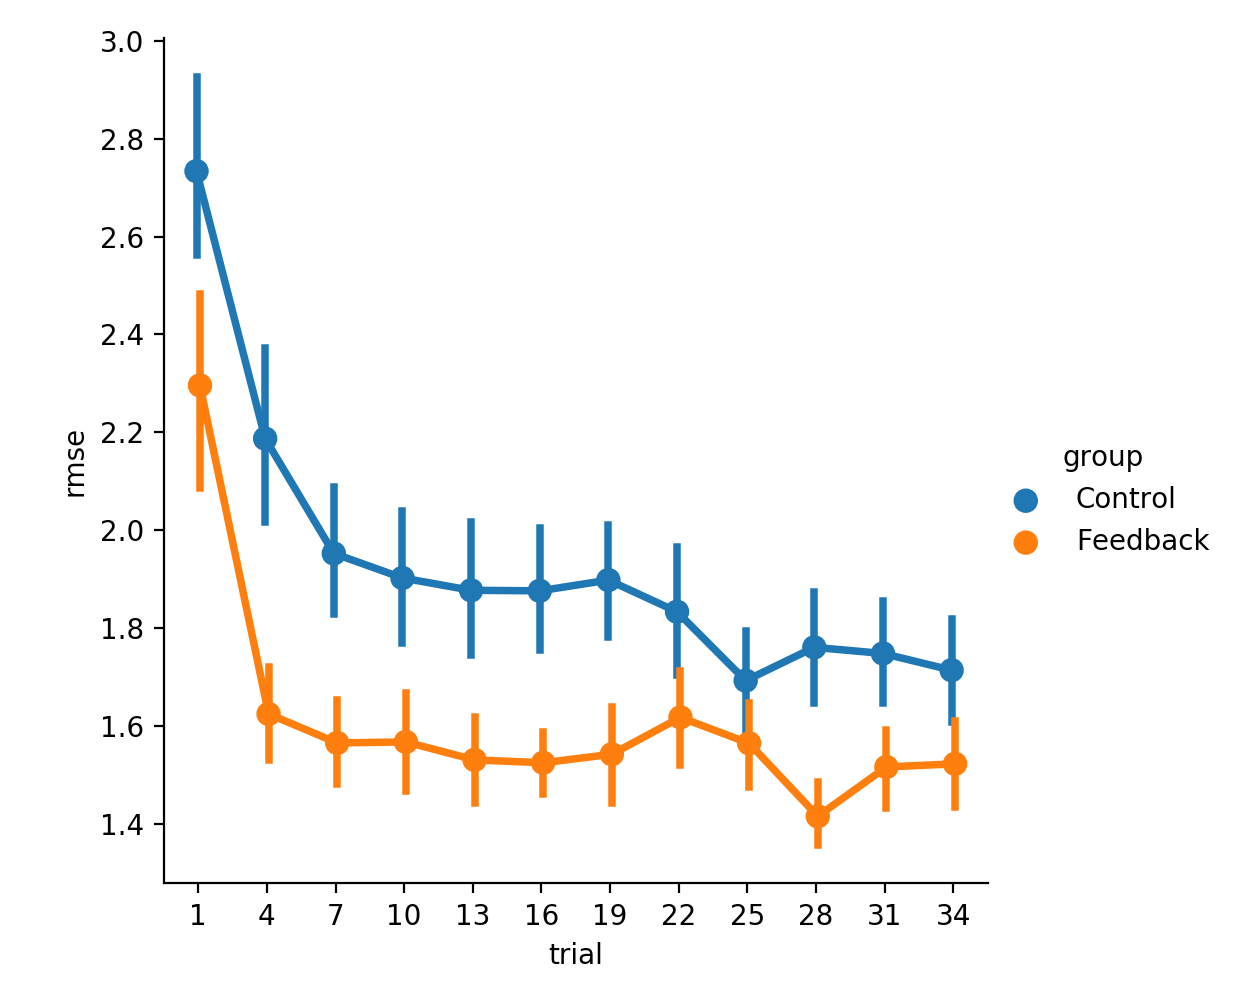
\includegraphics[width=3.25in]{figures/rmse.png}
        \caption{Root-mean-square-error}
        \label{fig:sm_rmse}
    \end{subfigure}
    \caption{Identified crossover frequency and predicted RMSE.}
    %    \label{fig:goodnessoffit}
\end{figure}

\clearpage

\begin{figure}[t]
    \centering
    \begin{subfigure}[h]{0.49\textwidth}
        \centering
        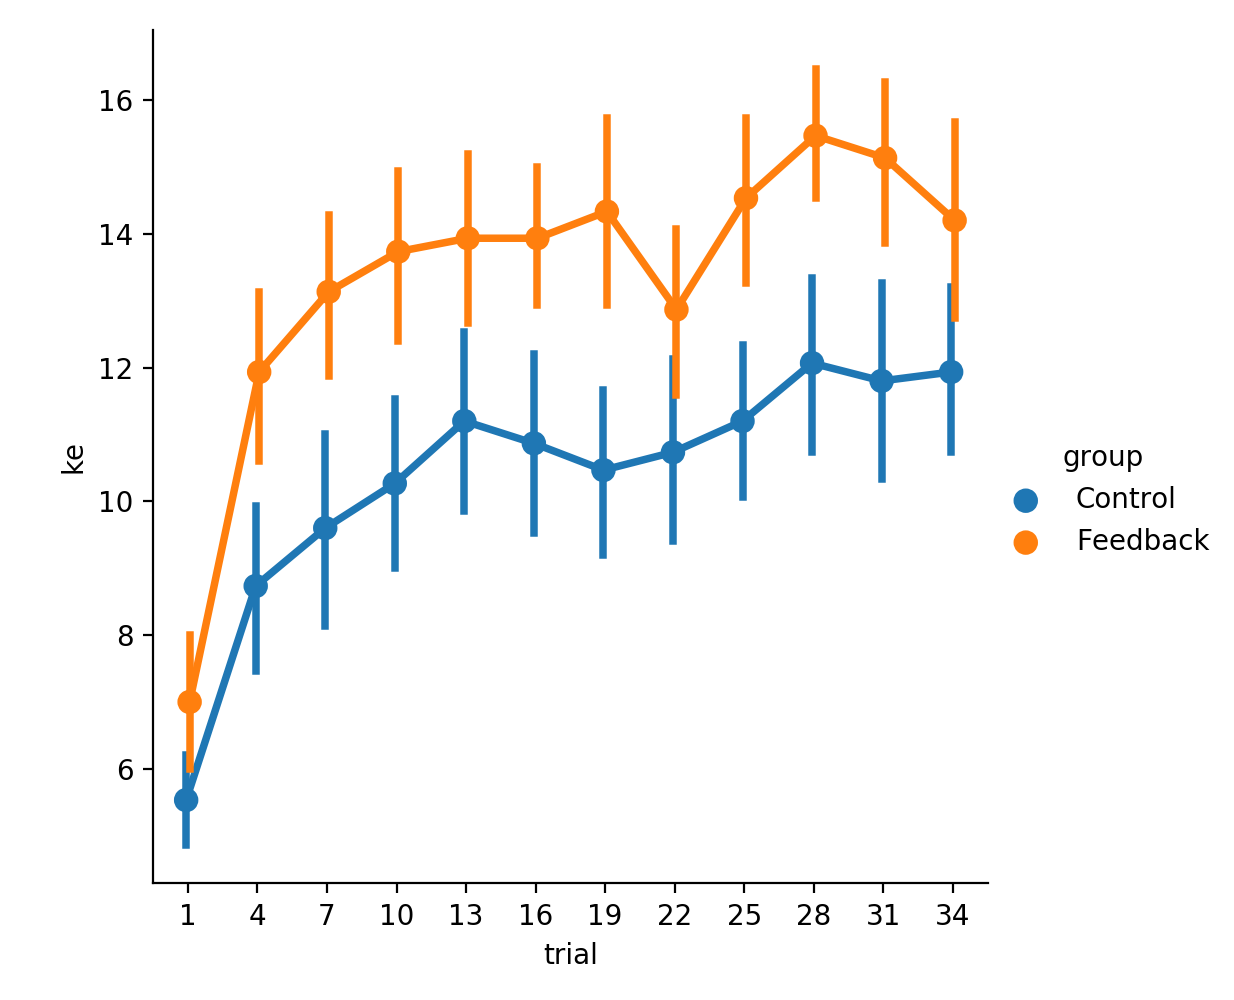
\includegraphics[width=3.25in]{figures/ke.png}
        \caption{$K_e$}
        \label{fig:sm_ke}
    \end{subfigure}
    \hfill
    \begin{subfigure}[h]{0.49\textwidth}
        \centering
        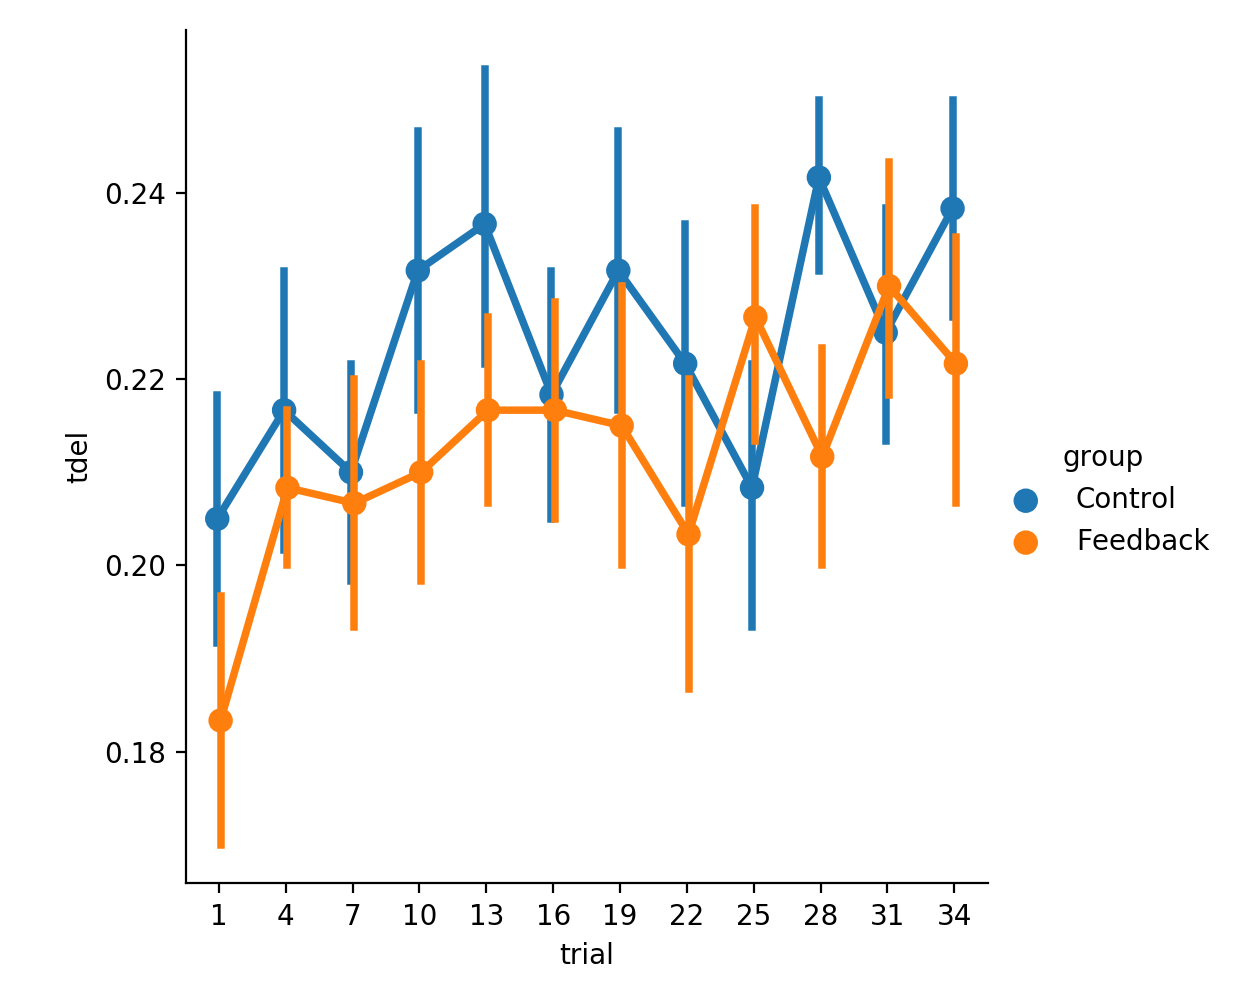
\includegraphics[width=3.25in]{figures/tdel.png}
        \caption{$\tau$}
        \label{fig:sm_tdel}
    \end{subfigure}
    \caption{Visual feedback outer loop.}
    %    \label{fig:goodnessoffit}
\end{figure}

\begin{figure}[t]
    \centering
    \begin{subfigure}[h]{0.49\textwidth}
        \centering
        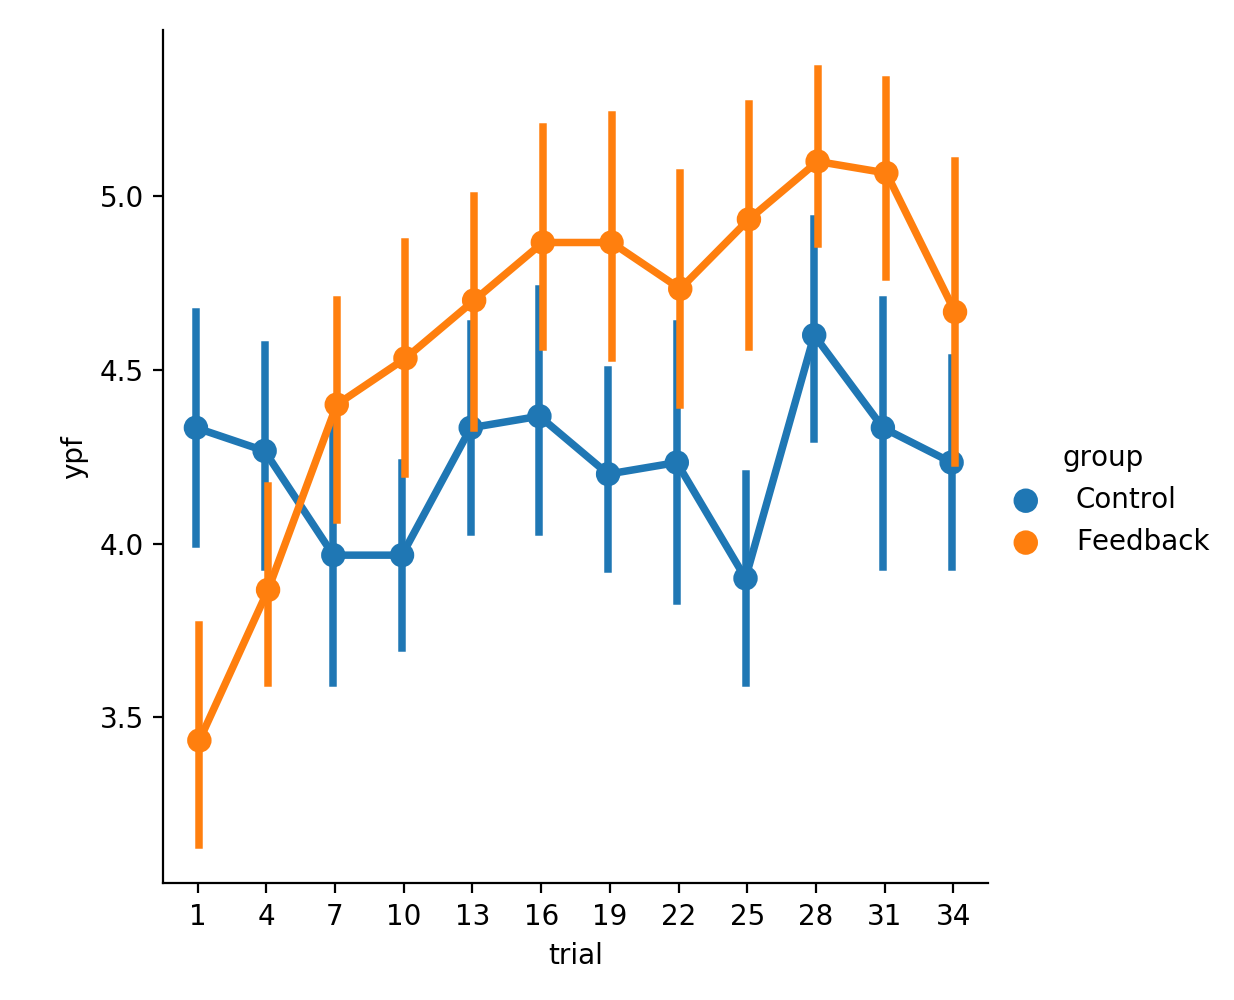
\includegraphics[width=3.25in]{figures/ypf.png}
        \caption{$K_{PF}$}
        \label{fig:sm_ypf}
    \end{subfigure}
    \hfill
    \begin{subfigure}[h]{0.49\textwidth}
        \centering
        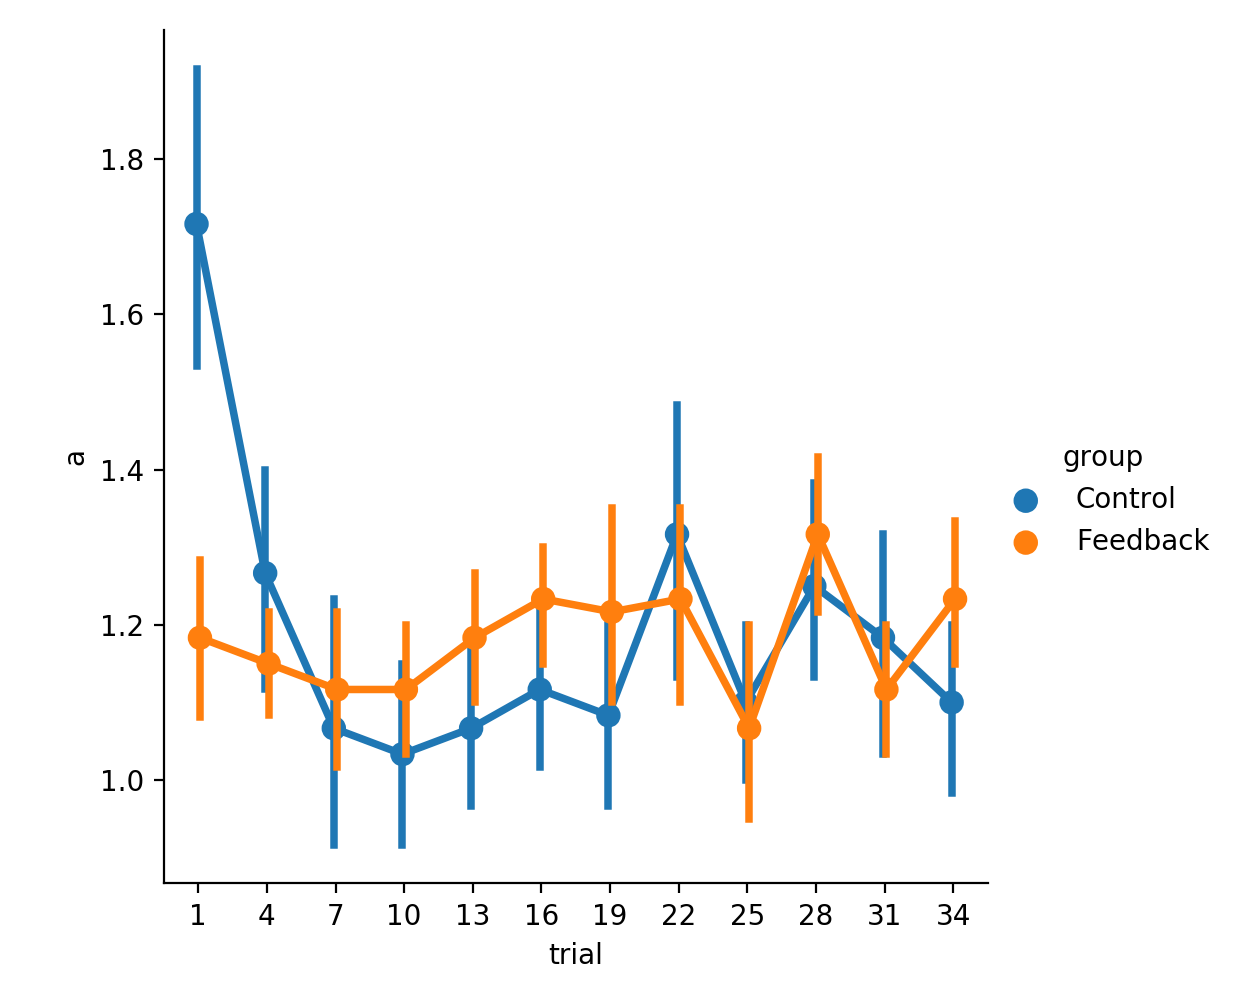
\includegraphics[width=3.25in]{figures/a.png}
        \caption{$a$}
        \label{fig:sm_a}
    \end{subfigure}
    \caption{Proprioceptive feedback inner loop.}
    %    \label{fig:goodnessoffit}
\end{figure}

% Structural Model Parameter Identification Technique

% 	Run (Parallel)ModelGenerator.m in MATLAB to generate many model outputs.
% 	Run ExperimentMatcher.py in Python to identify the global optimum best initial set of parameters.
% 	Run ModelOptimizer.m in MATLAB to iterate on the initial guess to identify an optimal set of parameters.
% 	Run ModelAnalysis.r in R to generate the statistics.
% 	Run OptimalModelPlots.py in Python to make the plots.

% Ke
% Type III Analysis of Variance Table with Satterthwaite's method
%       Sum Sq Mean Sq NumDF DenDF F value    Pr(>F)
% group  113.8  113.80     1    27  7.2654   0.01195 *
% trial 1493.7  135.79    11   308  8.6693 2.201e-13 ***
% ---
% Signif. codes:  0 ‘***’ 0.001 ‘**’ 0.01 ‘*’ 0.05 ‘.’ 0.1 ‘ ’ 1

% tdel
% Type III Analysis of Variance Table with Satterthwaite's method
%         Sum Sq   Mean Sq NumDF DenDF F value Pr(>F)
% group 0.000176 0.0001760     1    27  0.0171 0.8968
% trial 0.068712 0.0062466    11   308  0.6081 0.8217

% Ypf
% Type III Analysis of Variance Table with Satterthwaite's method
%       Sum Sq Mean Sq NumDF DenDF F value Pr(>F)
% group 12.032  12.032     1    27  1.6509 0.2097
% trial 82.819   7.529    11   308  1.0331 0.4168

% a
% Type III Analysis of Variance Table with Satterthwaite's method
%        Sum Sq Mean Sq NumDF DenDF F value   Pr(>F)
% group  0.0031 0.00314     1    27  0.0068 0.934953
% trial 13.6429 1.24026    11   308  2.6798 0.002657 **
% ---
% Signif. codes:  0 ‘***’ 0.001 ‘**’ 0.01 ‘*’ 0.05 ‘.’ 0.1 ‘ ’ 1

% Wnm
% Type III Analysis of Variance Table with Satterthwaite's method
%        Sum Sq Mean Sq NumDF DenDF F value Pr(>F)
% group   0.477  0.4768     1    27  0.0487 0.8270
% trial 130.831 11.8937    11   308  1.2141 0.2764

% Zetanm
% Type III Analysis of Variance Table with Satterthwaite's method
%          Sum Sq    Mean Sq NumDF DenDF F value  Pr(>F)
% group 0.0000331 0.00003309     1    27  0.1937 0.66338
% trial 0.0035074 0.00031886    11   308  1.8665 0.04314 *
% ---
% Signif. codes:  0 ‘***’ 0.001 ‘**’ 0.01 ‘*’ 0.05 ‘.’ 0.1 ‘ ’ 1


% All variables can be treated as constants with the exception of  K_e, which changes with both Trial and Group.
% tdel	Ypf	a	Wnm	Zetanm
% 0.238±0.006	5.927±0.163	1.301±0.041	7.768±0.185	0.707±0.001

% Model K_e as Exponential Fit: K_e=A*e^(-B*Trial)+C

% 	A	B	C
% Control	-7.34466243	0.37349137	12.40429001
% Feedback	-67.32338104	1.99463577	17.40238421

\section{Discussion}
% \begin{figure*}
%     \centering
%     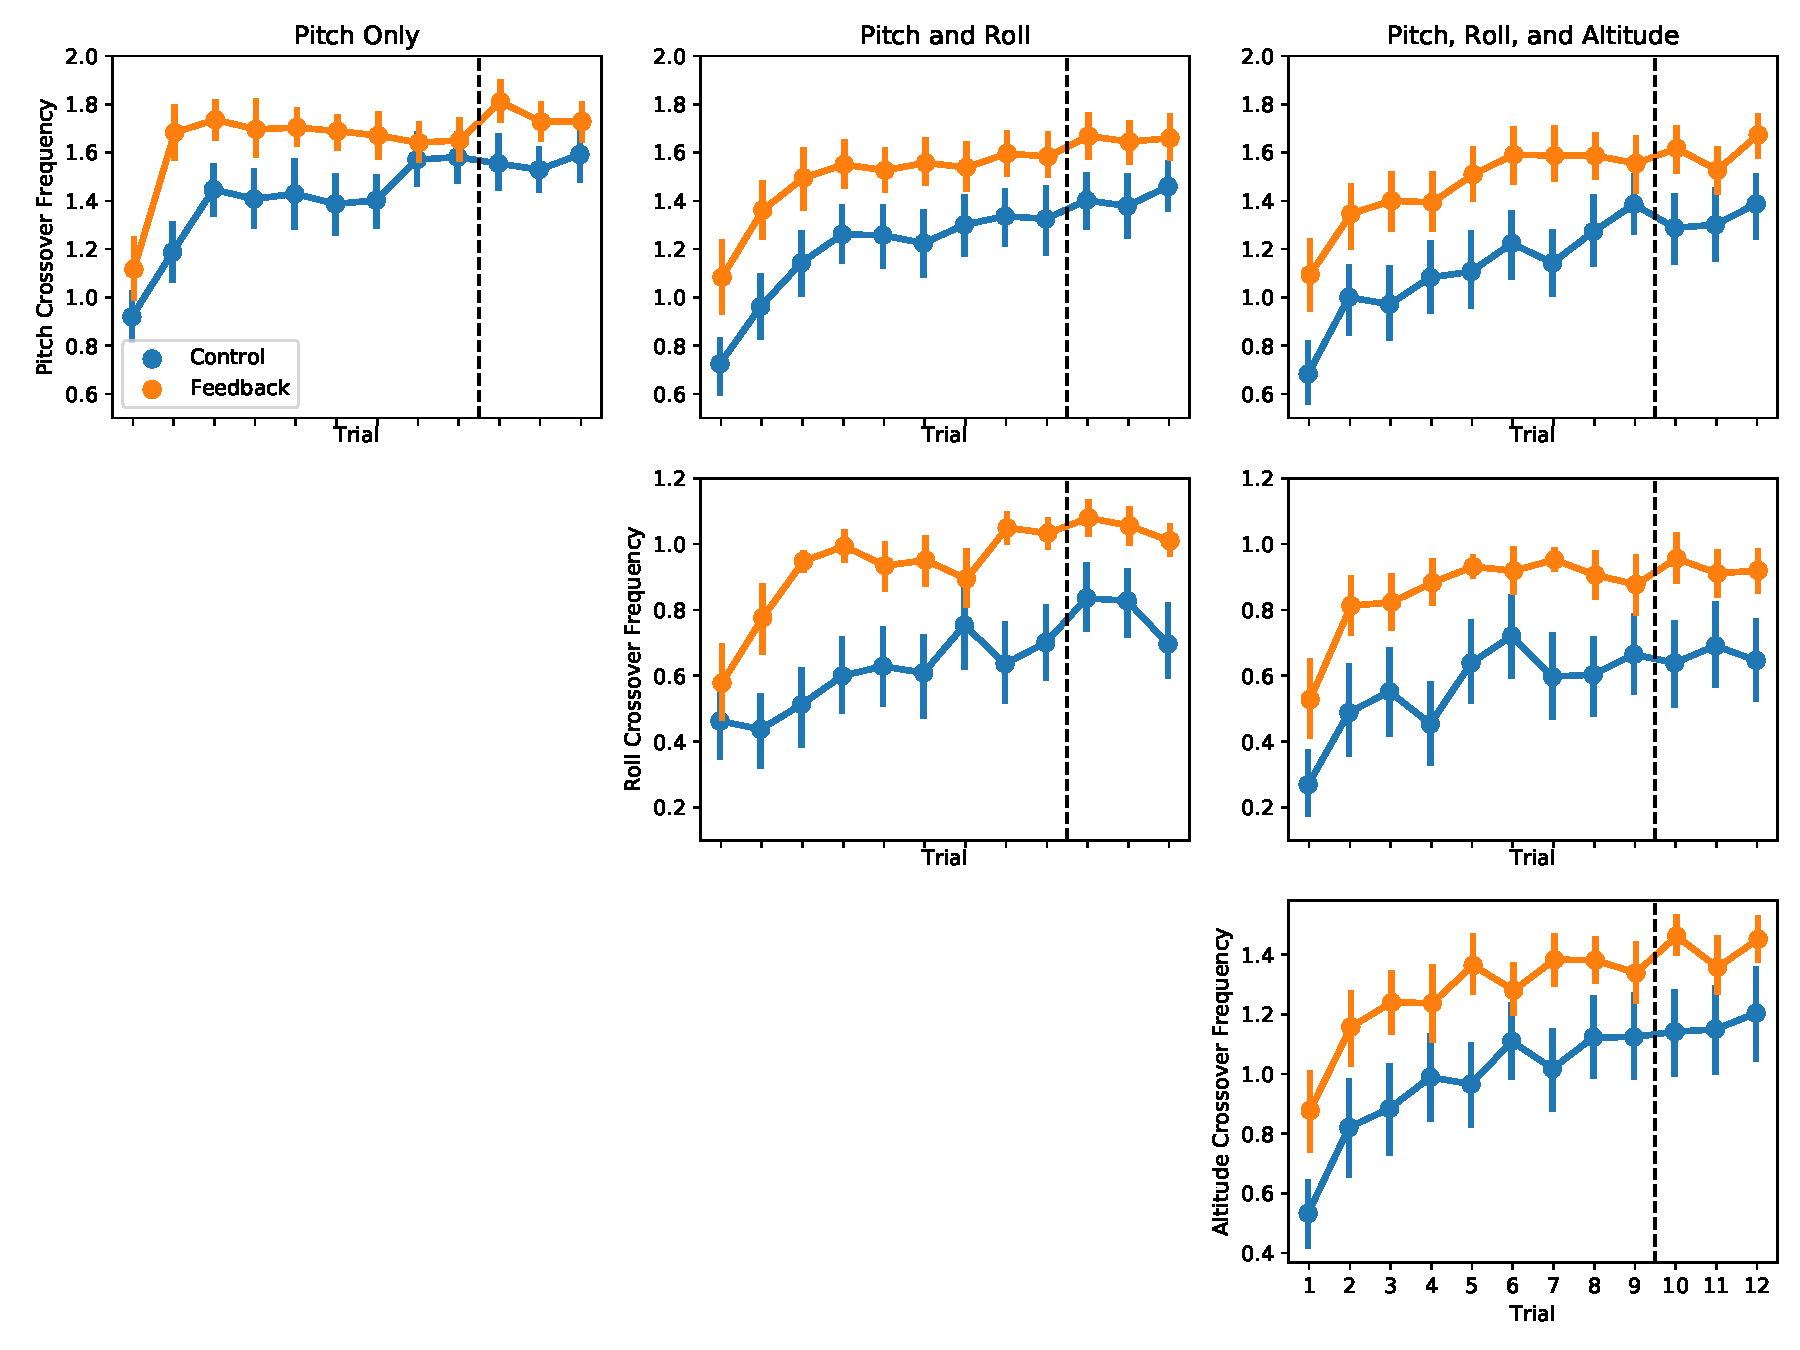
\includegraphics[width=6in]{figures/crossover_measures.pdf}
%     \caption{The crossover frequency of the estimated pilot/vehicle open-loop transfer functions for each group, trial, and control task.
%         The dashed line indicates where the feedback was removed from participants in the feedback group.
%         Error bars are the standard error of the mean.}
%     \label{figure:crossover_frequency_all}
% \end{figure*}

\begin{align*}
    \dot{\vec{x}}_{long} =
    \left[ \begin{array}{ *{5}{c} }
            X_u                     & X_w                     & X_q                                          & -g \cos \theta_0 & 0 \\
            Z_u                     & Z_w                     & Z_q + U_0                                    & -g \sin \theta_0 & 0 \\
            M_u + M_{\dot{w}} Z_{u} & M_w + M_{\dot{w}} Z_{w} & M_q + M_{\dot{w}} \left( Z_{q} + U_0 \right) & 0                & 0 \\
            0                       & 0                       & 1                                            & 0                & 0 \\
            0                       & -1                      & 0                                            & U_0              & 0 \\
        \end{array} \right]
    \left[ \begin{array}{ *{1}{c} }
            \Delta u      \\
            \Delta w      \\
            \Delta q      \\
            \Delta \theta \\
            \Delta z      \\
        \end{array} \right] & + \\
    \left[ \begin{array}{ *{5}{c} }
            X_{\delta_e}                            & X_{\delta_{th}}                               \\
            Z_{\delta_e}                            & Z_{\delta_{th}}                               \\
            M_{\delta_e} + M_{\dot{w}} Z_{\delta_e} & M_{\delta_{th}} + M_{\dot{w}} Z_{\delta_{th}} \\
            0                                       & 0                                             \\
            0                                       & 0                                             \\
        \end{array} \right]
    \left[ \begin{array}{ *{1}{c} }
            \Delta \delta_e    \\
            \Delta \delta_{th} \\
        \end{array} \right] &   \\
\end{align*}

\begin{align*}
    \dot{\vec{x}}_{lat} =
    \left[ \begin{array}{ *{5}{c} }
            Y_v  & Y_p  & Y_r - U_0     & g \cos \theta_0  & 0 \\
            L'_v & L'_p & L'_r          & -g \sin \theta_0 & 0 \\
            N'_v & N'_p & N'_r          & 0                & 0 \\
            0    & 1    & \tan \theta_0 & 0                & 0 \\
            0    & 0    & \sec \theta_0 & 0                & 0 \\
        \end{array} \right]
    \left[ \begin{array}{ *{1}{c} }
            \Delta v    \\
            \Delta p    \\
            \Delta r    \\
            \Delta \phi \\
            \Delta \psi \\
        \end{array} \right] & + \\
    \left[ \begin{array}{ *{5}{c} }
            Y_{\delta_{a}}  & Y_{\delta_{r}}  \\
            L'_{\delta_{a}} & L'_{\delta_{r}} \\
            N'_{\delta_{a}} & N'_{\delta_{r}} \\
            0               & 0               \\
            0               & 0               \\
        \end{array} \right]
    \left[ \begin{array}{ *{1}{c} }
            \Delta \delta_a \\
            \Delta \delta_r \\
        \end{array} \right] &   \\
\end{align*}
